\chapter{ANALYSE DES RESULTATS OBTENUS ET DISCUSSIONS}
\thispagestyle{empty}
\label{chap:analyse-resultats-discussions}

\section{Cadre general de l'analyse}

Cette partie analyse les resultats experimentaux obtenus dans l'evaluation complete des modeles de resume multilingue. Les resultats utilises proviennent du repertoire \texttt{evaluation/xlsum\_eval\_full}. L'evaluation a ete realisee sur le split \texttt{test} de \texttt{csebuetnlp/xlsum}, avec 52.219 exemples repartis sur 11 langues executables: arabe, anglais, espagnol, francais, hindi, japonais, coreen, russe, turc, vietnamien et chinois simplifie. Les langues allemand, italien, neerlandais et roumain, prevues dans le plan initial, n'ont pas ete evaluees car les sous-ensembles publics correspondants n'etaient pas disponibles dans la version locale de XL-Sum.

Il faut donc distinguer la couverture experimentale et la couverture applicative. Les donnees d'entrainement et d'evaluation disponibles dans XL-Sum couvrent 11 langues dans cette execution, mais l'application finale conserve un support de resume pour 15 langues. Les quatre langues non evaluees quantitativement, c'est-a-dire l'allemand, l'italien, le neerlandais et le roumain, peuvent encore etre traitees dans le flux applicatif par les modeles multilingues lorsque le code de langue et la tokenisation du modele le permettent. En revanche, aucune conclusion numerique solide n'est tiree pour ces quatre langues, car elles ne disposent pas ici d'un split XL-Sum comparable.

Trois modeles sont compares. Les modeles \texttt{mbart50\_\allowbreak xlsum} et \texttt{mbart-\allowbreak xlsum-2} sont les deux modeles mBART entraines dans le cadre du projet. Le modele \texttt{mt5-\allowbreak xlsum} est utilise comme modele de comparaison pret a l'emploi. Il ne doit donc pas etre interprete comme une sortie directe de l'entrainement du projet, mais comme une reference forte pour situer la performance des modeles mBART.

Les metriques interpretees dans cette section couvrent trois familles. La premiere regroupe les metriques classiques de recouvrement avec le resume de reference, notamment ROUGE-L, BLEU et METEOR-lite. La deuxieme regroupe les metriques de comportement, comme la couverture de la source, le taux de compression, la nouveaute et la latence. La troisieme regroupe les scores proxy composites definis dans la pipeline d'evaluation: coherence, exactitude, clarte, pertinence, efficacite et score global de capacite. Ces scores automatiques ne remplacent pas une evaluation humaine, mais ils permettent une comparaison reproductible des modeles dans les memes conditions experimentales.

\begin{table}[t]
\caption{Synthese macro des resultats sur XL-Sum test}
\label{tab:analyse-overall-summary}
\centering
\begin{tabular}{|l|r|r|r|r|r|r|}
\hline
\textbf{Modele} & \textbf{Cap.} & \textbf{R-L} & \textbf{BLEU} & \textbf{METEOR} & \textbf{Fact.} & \textbf{Lat.} \\
\hline
\texttt{mt5-\allowbreak xlsum} & 0.6631 & 0.3010 & 0.1310 & 0.3195 & 0.8522 & 0.2552 \\
\hline
\texttt{mbart50\_\allowbreak xlsum} & 0.6578 & 0.2785 & 0.1202 & 0.3157 & 0.8522 & 0.1917 \\
\hline
\texttt{mbart-\allowbreak xlsum-2} & 0.6570 & 0.2792 & 0.1228 & 0.3181 & 0.8249 & 0.1840 \\
\hline
\end{tabular}
\end{table}

Le Tableau~\ref{tab:analyse-overall-summary} montre que les trois modeles restent proches en score global de capacite. \texttt{mt5-\allowbreak xlsum} obtient la meilleure moyenne globale, avec 0.6631. Les deux modeles mBART suivent avec 0.6578 et 0.6570. L'ecart absolu entre le meilleur modele et le meilleur modele entraine dans le projet est donc d'environ 0.0053, ce qui indique une proximite globale malgre des profils de comportement differents.

\section{Classement global des modeles}

La Figure~\ref{fig:analyse-overall-rank-heatmap} resume le rang de chaque modele selon les principales metriques. Elle confirme que le classement n'est pas uniforme: \texttt{mt5-\allowbreak xlsum} domine les metriques classiques de similarite avec la reference, tandis que les modeles mBART sont plus competitifs sur l'efficacite et certains indicateurs de comportement.

\begin{figure}[t]
\centering
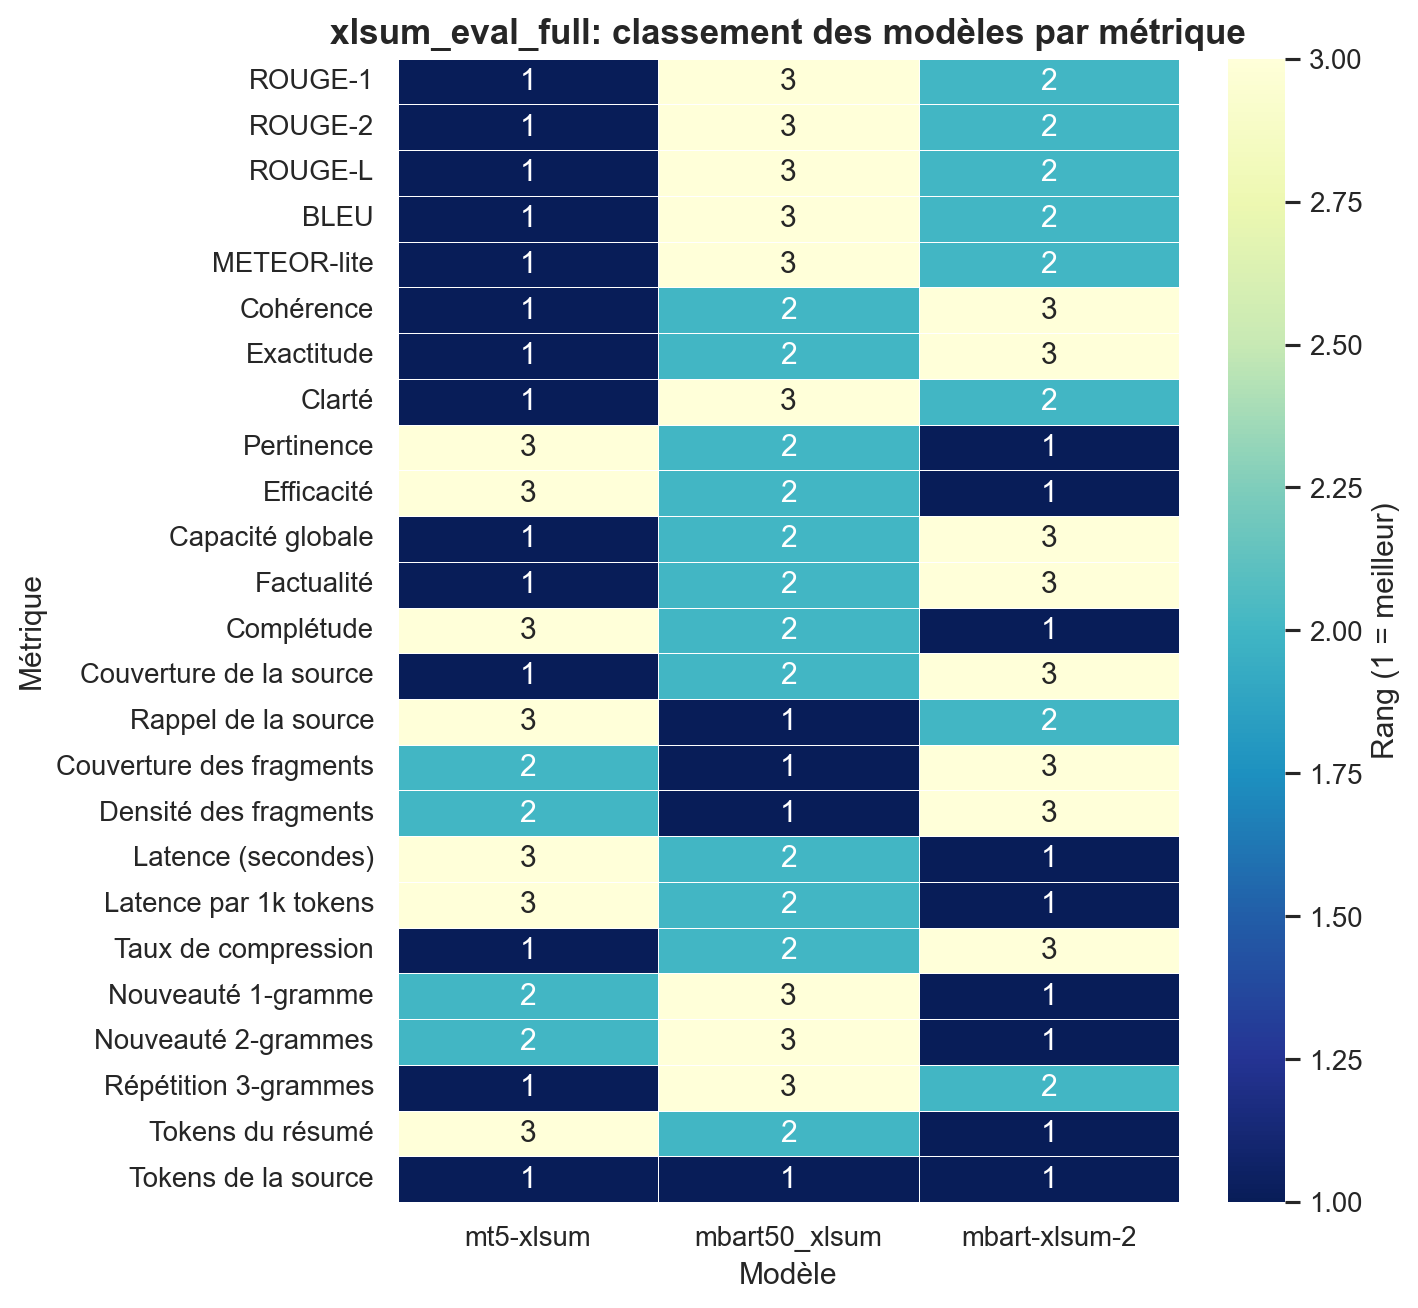
\includegraphics[width=.95\linewidth]{figures/analyse/overall_rank_heatmap.png}
\caption{Classement global des modeles selon les metriques principales}
\label{fig:analyse-overall-rank-heatmap}
\end{figure}

Le principal avantage de \texttt{mt5-\allowbreak xlsum} concerne la similarite avec les resumes humains. Il obtient les meilleures valeurs en ROUGE-L, BLEU et METEOR-lite. Cela signifie que ses sorties recouvrent davantage les formulations et le contenu lexical des references XL-Sum. Ce resultat est coherent avec son role de modele de reference deja adapte a XL-Sum.

Les deux modeles mBART presentent un profil different. \texttt{mbart50\_\allowbreak xlsum} atteint un score global tres proche de \texttt{mt5-\allowbreak xlsum} tout en etant plus rapide. Il conserve aussi une forte fidelite a la source: son score de factualite est pratiquement identique a celui de \texttt{mt5-\allowbreak xlsum}. \texttt{mbart-\allowbreak xlsum-2} est le modele le plus rapide en moyenne et obtient la meilleure completude automatique, mais il perd une partie de la couverture source. Son comportement est donc plus abstractive, avec un gain leger en BLEU, METEOR-lite et completude par rapport a \texttt{mbart50\_\allowbreak xlsum}, mais avec une baisse de l'ancrage direct dans le texte source.

La moyenne globale doit cependant etre completee par une lecture par langue. Le Tableau~\ref{tab:analyse-language-winners} montre que \texttt{mt5-\allowbreak xlsum} est premier dans 7 langues, tandis que \texttt{mbart50\_\allowbreak xlsum} est premier dans 4 langues. \texttt{mbart-\allowbreak xlsum-2} n'est pas premier selon le score global de capacite, mais il reste proche du meilleur modele dans plusieurs langues, notamment en hindi, vietnamien et chinois simplifie.

\begin{table}[t]
\caption{Meilleur modele par langue selon le score global de capacite}
\label{tab:analyse-language-winners}
\centering
\begin{tabular}{|l|l|r|l|r|}
\hline
\textbf{Langue} & \textbf{Meilleur} & \textbf{Cap.} & \textbf{Deuxieme} & \textbf{Ecart} \\
\hline
arabe & \texttt{mbart50} & 0.6403 & \texttt{mt5} & 0.0021 \\
\hline
anglais & \texttt{mbart50} & 0.6255 & \texttt{mbart-2} & 0.0022 \\
\hline
espagnol & \texttt{mt5} & 0.6725 & \texttt{mbart50} & 0.0026 \\
\hline
francais & \texttt{mbart50} & 0.6463 & \texttt{mt5} & 0.0005 \\
\hline
hindi & \texttt{mt5} & 0.6544 & \texttt{mbart-2} & 0.0041 \\
\hline
japonais & \texttt{mt5} & 0.6977 & \texttt{mbart50} & 0.0106 \\
\hline
coreen & \texttt{mt5} & 0.7334 & \texttt{mbart50} & 0.0095 \\
\hline
russe & \texttt{mbart50} & 0.6385 & \texttt{mbart-2} & 0.0028 \\
\hline
turc & \texttt{mt5} & 0.6278 & \texttt{mbart50} & 0.0092 \\
\hline
vietnamien & \texttt{mt5} & 0.6524 & \texttt{mbart-2} & 0.0043 \\
\hline
chinois simplifie & \texttt{mt5} & 0.7134 & \texttt{mbart-2} & 0.0158 \\
\hline
\end{tabular}
\end{table}

Cette table montre que les ecarts sont parfois tres faibles. En francais, par exemple, \texttt{mbart50} devance \texttt{mt5} de seulement 0.0005. En anglais, les trois modeles sont egalement tres proches. A l'inverse, l'avantage de \texttt{mt5} est plus net en chinois simplifie, japonais, coreen et turc. Pour cette raison, le choix du modele ne doit pas etre fait uniquement a partir de la moyenne macro, mais aussi selon la langue cible.

La Figure~\ref{fig:analyse-latency-capability-tradeoff} illustre le compromis entre latence moyenne et capacite globale. Le point le plus haut correspond a \texttt{mt5-\allowbreak xlsum}, mais il est aussi plus lent. Les deux mBART sont situes plus a gauche, ce qui correspond a un temps moyen plus faible. Ce resultat est important pour l'application, car la generation des resumes doit rester exploitable dans un flux d'actualites multilingue.

\begin{figure}[t]
\centering
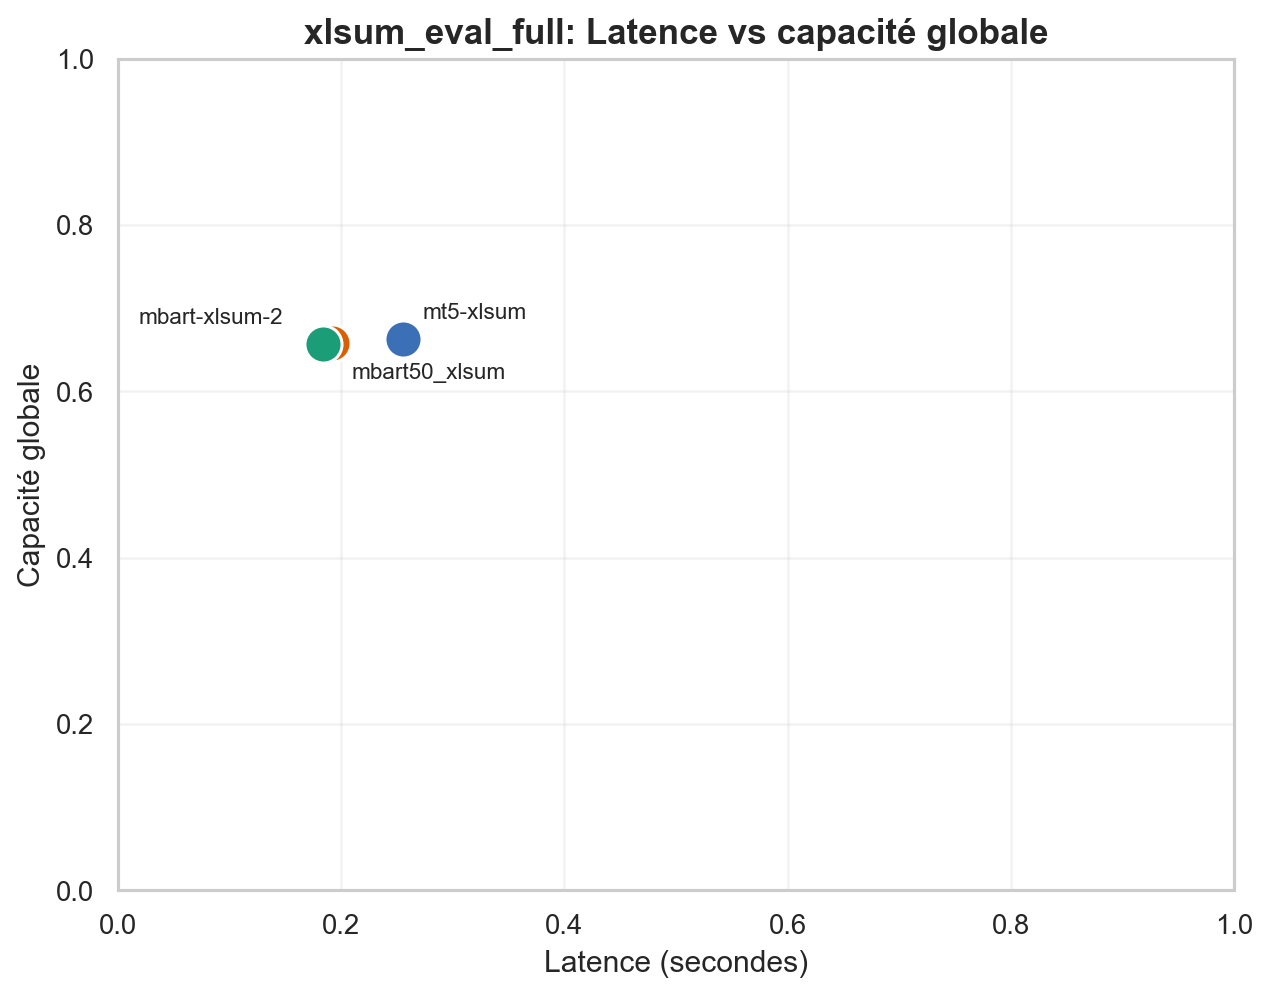
\includegraphics[width=.92\linewidth]{figures/analyse/overall_tradeoff_latency_seconds_mean__capability_overall_mean.png}
\caption{Compromis entre latence moyenne et capacite globale}
\label{fig:analyse-latency-capability-tradeoff}
\end{figure}

\section{Compression, completude et abstraction}

Le taux de compression et la completude montrent un autre compromis. \texttt{mt5-\allowbreak xlsum} produit en moyenne des resumes plus courts: son taux de compression moyen est 27.13, contre 23.25 pour \texttt{mbart50\_\allowbreak xlsum} et 23.10 pour \texttt{mbart-\allowbreak xlsum-2}. En revanche, les deux modeles mBART obtiennent une completude legerement superieure: 0.4525 pour \texttt{mbart50\_\allowbreak xlsum} et 0.4576 pour \texttt{mbart-\allowbreak xlsum-2}, contre 0.4489 pour \texttt{mt5-\allowbreak xlsum}.

\begin{figure}[t]
\centering
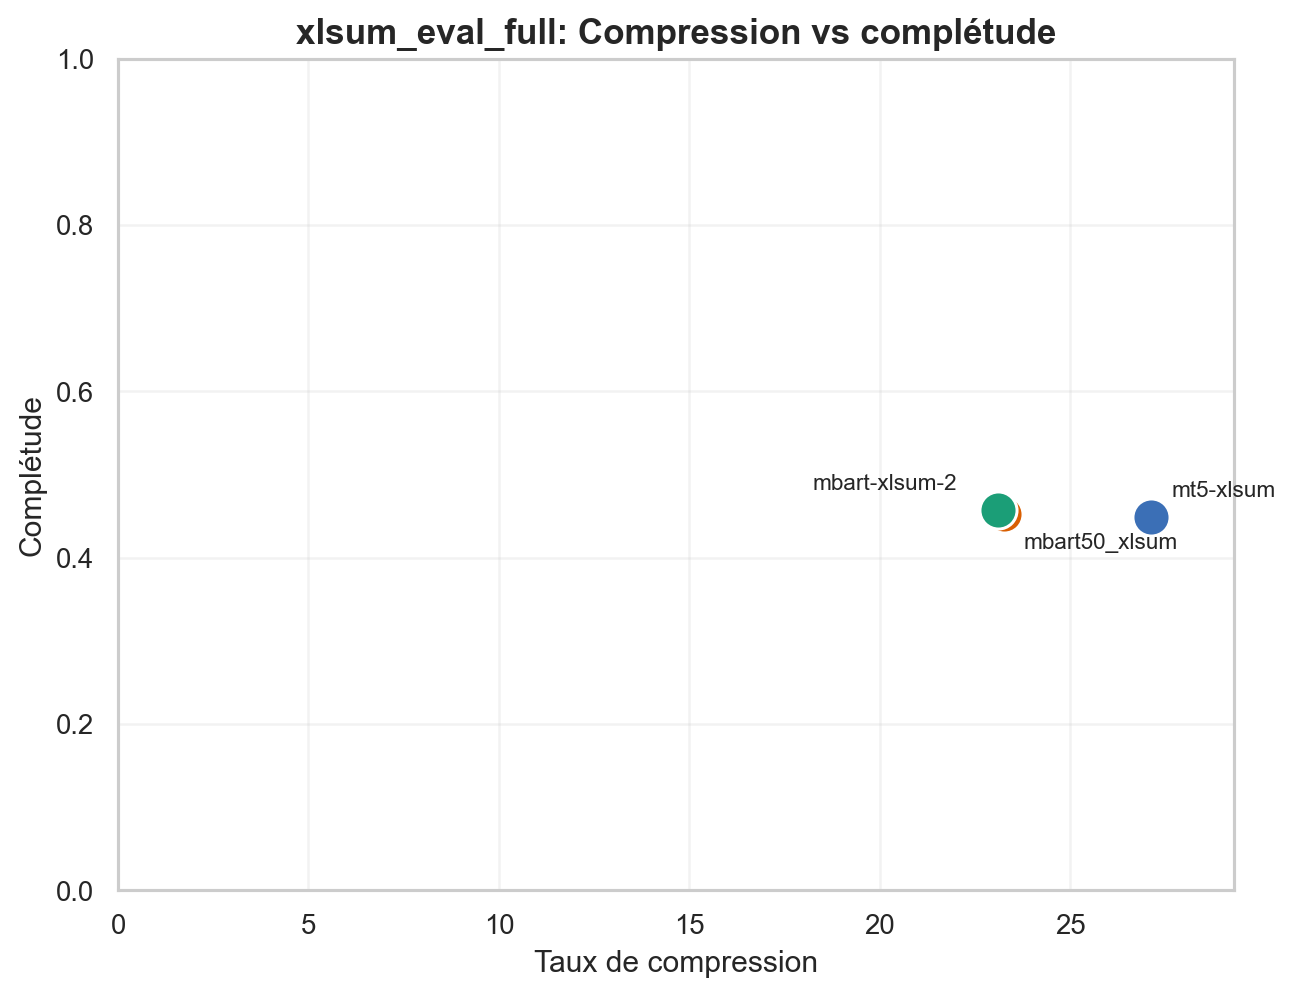
\includegraphics[width=.92\linewidth]{figures/analyse/overall_tradeoff_compression_ratio_mean__quality_completeness_mean.png}
\caption{Compromis entre taux de compression et completude automatique}
\label{fig:analyse-compression-completeness-tradeoff}
\end{figure}

La Figure~\ref{fig:analyse-compression-completeness-tradeoff} montre que la compression plus forte ne conduit pas automatiquement a une meilleure completude. \texttt{mt5-\allowbreak xlsum} est plus concis, mais les modeles mBART gardent legerement plus de contenu selon le score de completude. Dans le contexte du projet, ce resultat est utile: un resume d'actualite ne doit pas seulement etre court, il doit aussi conserver les informations essentielles de l'article.

La difference entre les deux mBART est egalement significative. \texttt{mbart-\allowbreak xlsum-2} a ete entraine avec une cible plus courte et une strategie de validation plus orientee qualite. Pourtant, il produit en moyenne un nombre de tokens proche de \texttt{mbart50\_\allowbreak xlsum} et obtient une meilleure completude. En parallele, sa nouveaute 2-grammes atteint 0.4712, contre 0.4229 pour \texttt{mbart50\_\allowbreak xlsum}. Cela indique que le deuxieme modele reformule davantage. Cette abstraction peut ameliorer la qualite percue lorsque la reformulation reste correcte, mais elle augmente aussi le risque de s'eloigner de la source.

\section{Analyse de la latence par langue}

Les cartes thermiques de latence permettent d'observer si le cout de generation est uniforme selon les langues. La Figure~\ref{fig:analyse-language-latency-seconds} presente la latence moyenne en secondes pour chaque couple langue-modele, tandis que la Figure~\ref{fig:analyse-language-latency-per-1k} normalise cette valeur par 1.000 tokens source.

\begin{figure}[t]
\centering
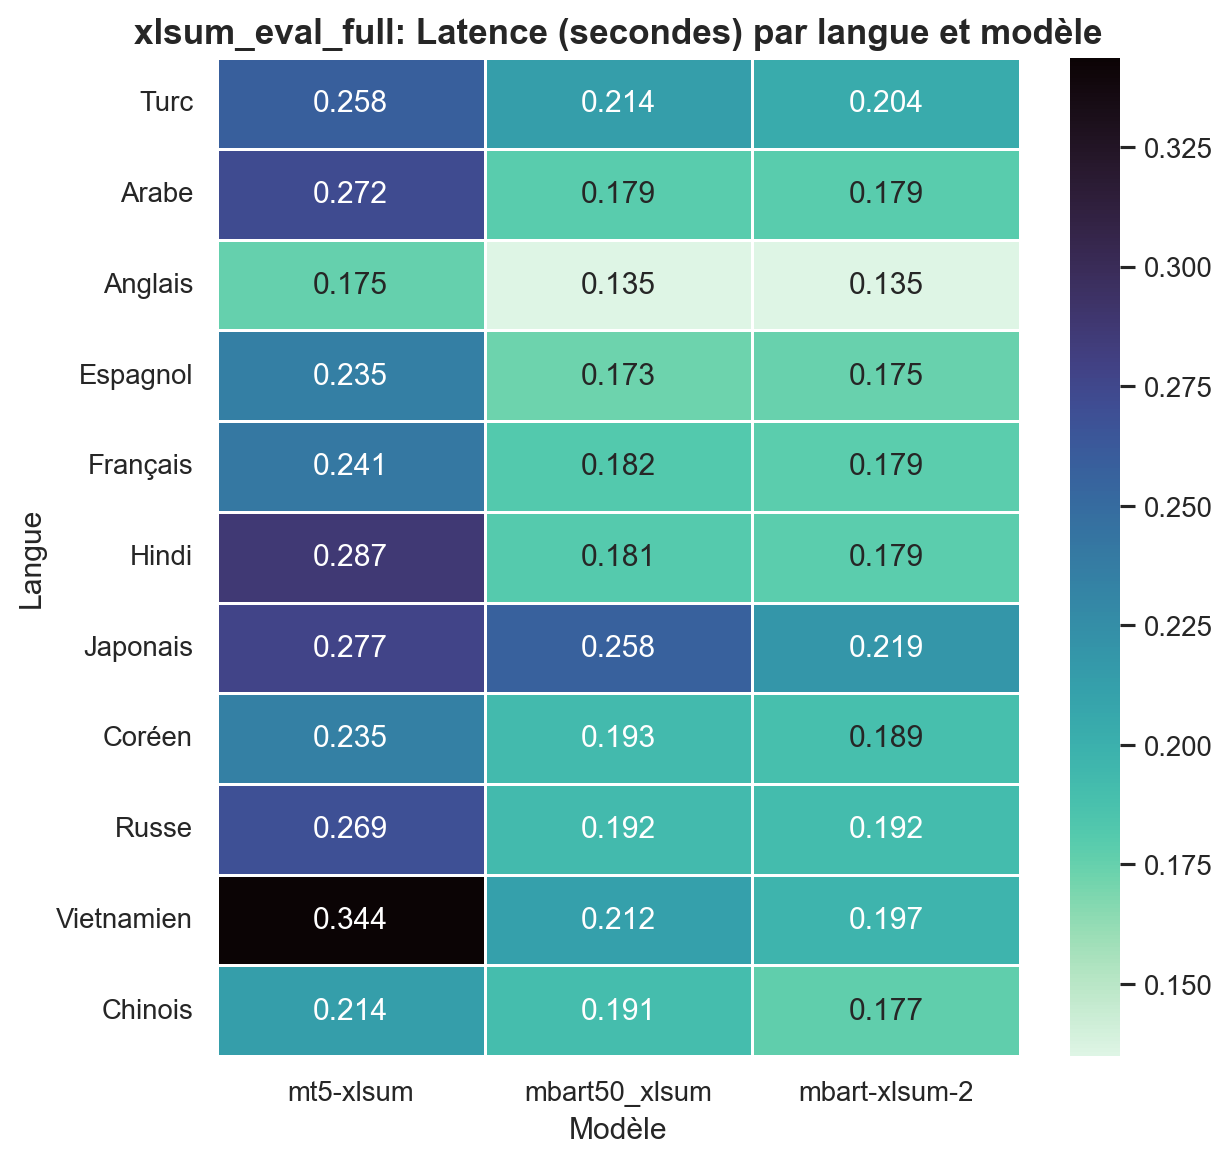
\includegraphics[width=.90\linewidth]{figures/analyse/language_model_heatmap_latency_seconds_mean.png}
\caption{Latence moyenne par langue et par modele}
\label{fig:analyse-language-latency-seconds}
\end{figure}

\begin{figure}[t]
\centering
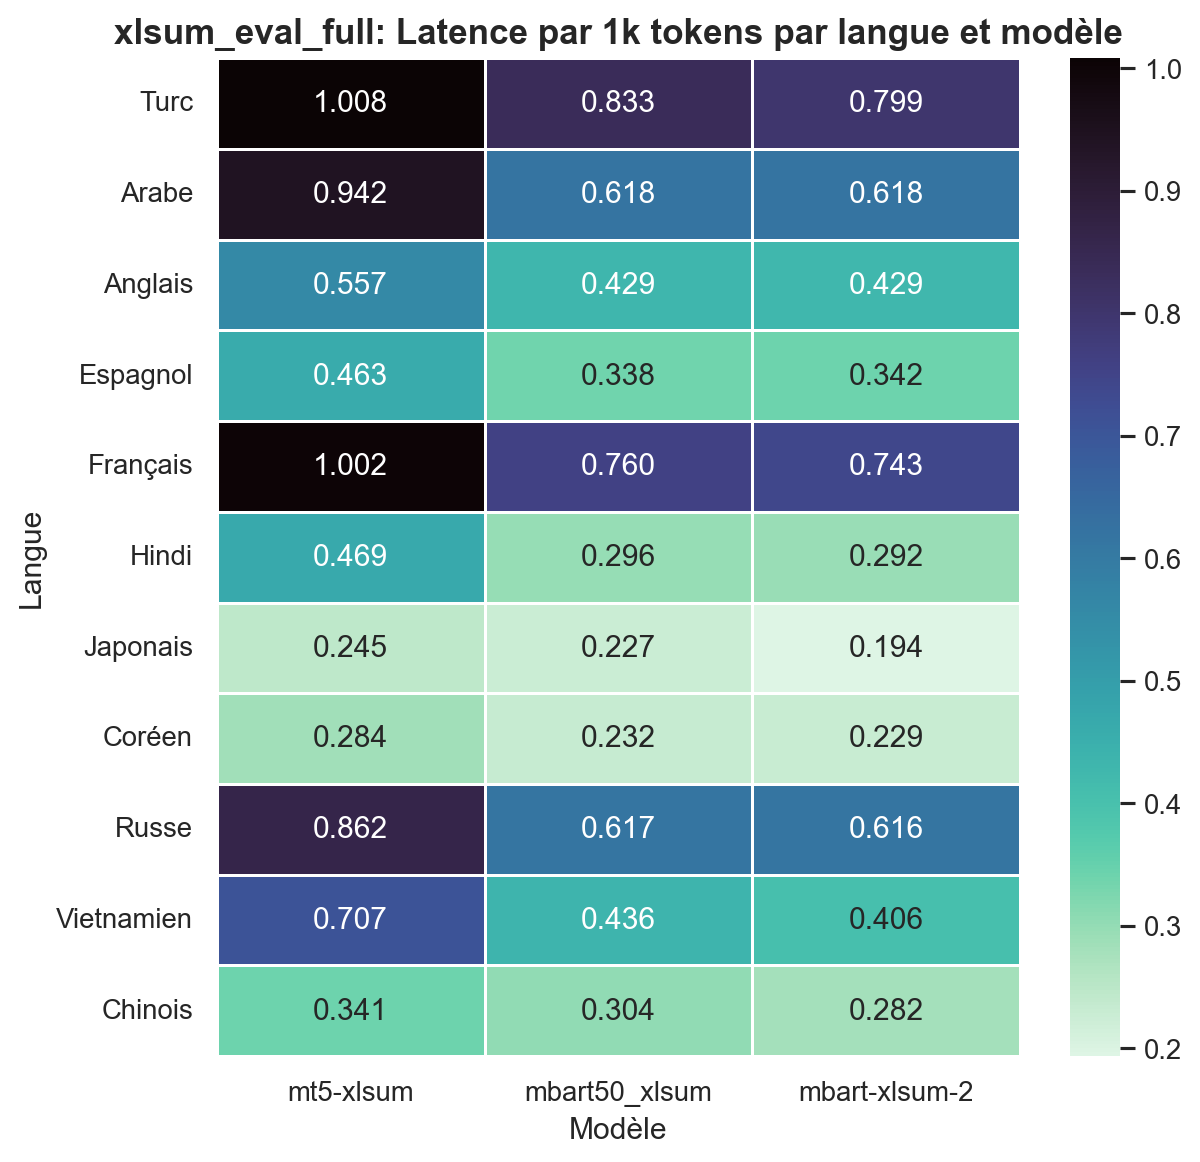
\includegraphics[width=.90\linewidth]{figures/analyse/language_model_heatmap_latency_per_1k_tokens_mean.png}
\caption{Latence moyenne normalisee par 1.000 tokens source}
\label{fig:analyse-language-latency-per-1k}
\end{figure}

La latence brute depend a la fois du modele, de la langue et de la longueur moyenne des articles. Les langues comme le japonais, le coreen et le chinois ont des textes sources plus longs dans le split test, ce qui peut augmenter le temps absolu de generation. La normalisation par 1.000 tokens permet donc de mieux comparer l'efficacite propre du modele. Dans les deux vues, \texttt{mbart-\allowbreak xlsum-2} et \texttt{mbart50\_\allowbreak xlsum} restent generalement plus rapides que \texttt{mt5-\allowbreak xlsum}.

Cette difference se voit aussi dans la distribution cumulative de la latence. La Figure~\ref{fig:analyse-ecdf-latency} montre que les courbes des modeles mBART sont deplacees vers les temps plus faibles. Au niveau des exemples, le modele le plus rapide est \texttt{mbart-\allowbreak xlsum-2} dans 51.4\% des cas et \texttt{mbart50\_\allowbreak xlsum} dans 47.2\% des cas. \texttt{mt5-\allowbreak xlsum} n'est le plus rapide que dans 1.4\% des cas.

\begin{figure}[t]
\centering
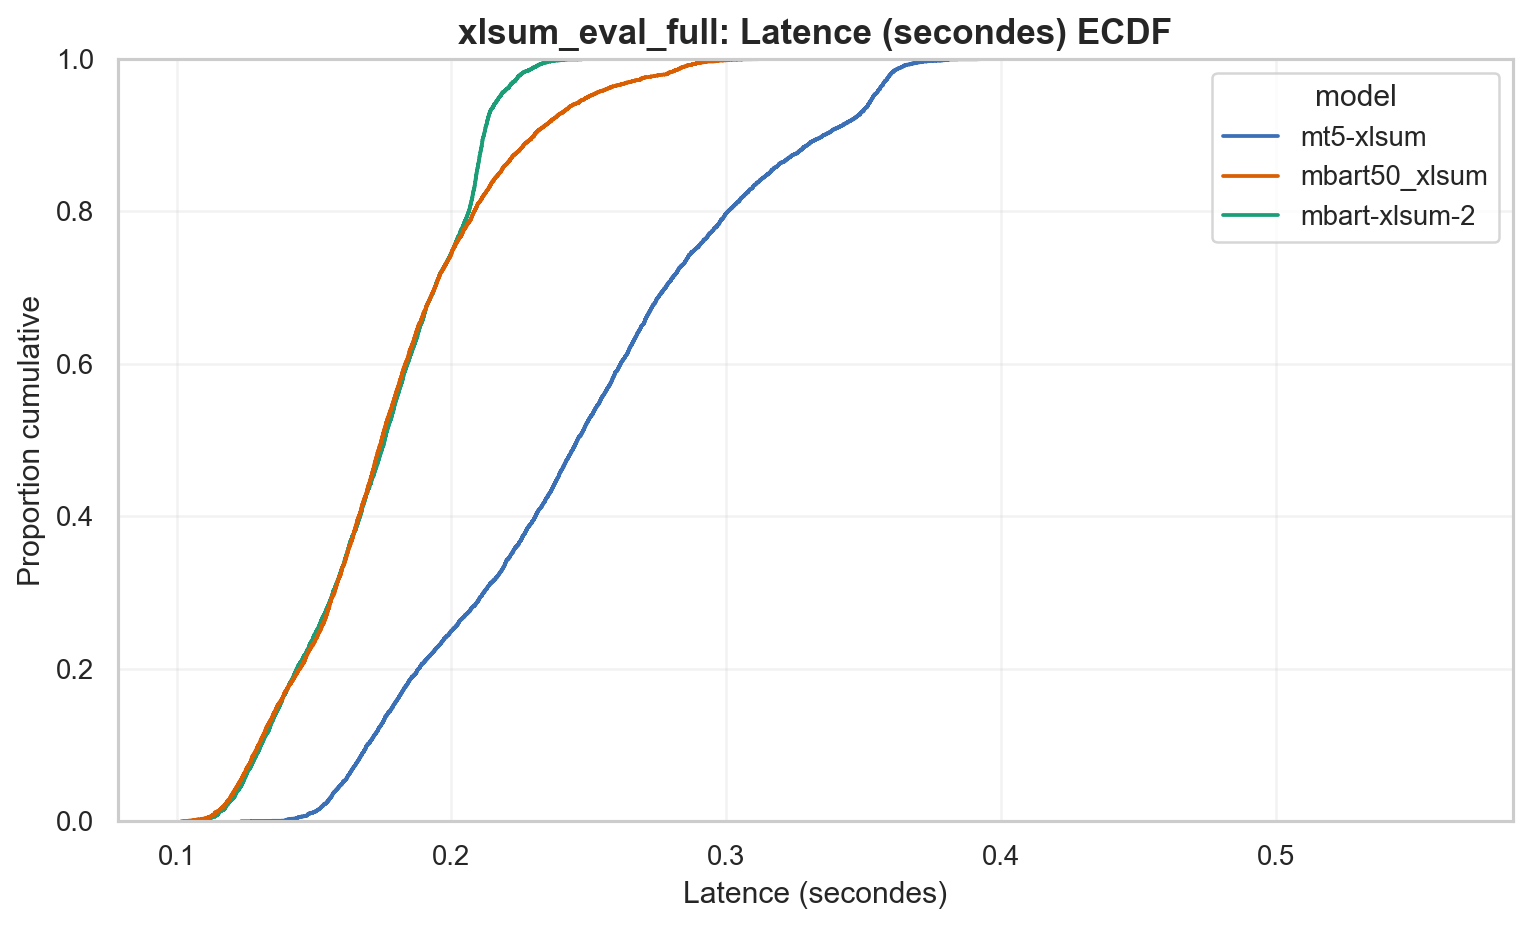
\includegraphics[width=.92\linewidth]{figures/analyse/ecdf_latency_seconds.png}
\caption{Distribution cumulative empirique de la latence}
\label{fig:analyse-ecdf-latency}
\end{figure}

Pour l'application web, cette observation justifie l'utilisation d'une generation en arriere-plan et d'un stockage des resumes en base. Meme si les temps moyens semblent faibles dans l'environnement d'evaluation, la multiplication par le nombre d'articles, de langues et de modeles rend la latence importante a l'echelle du systeme.

\section{Relations entre les metriques}

La Figure~\ref{fig:analyse-correlation-all-metrics} presente les correlations entre les metriques numeriques. Cette figure aide a comprendre pourquoi un modele peut etre premier selon une metrique et moins bon selon une autre. Les metriques classiques de recouvrement sont naturellement liees entre elles, car elles mesurent toutes une forme de proximite avec le resume de reference. En revanche, les metriques de source, de nouveaute, de compression et de latence capturent des comportements differents.

\begin{figure}[p]
\centering
\vspace*{\fill}
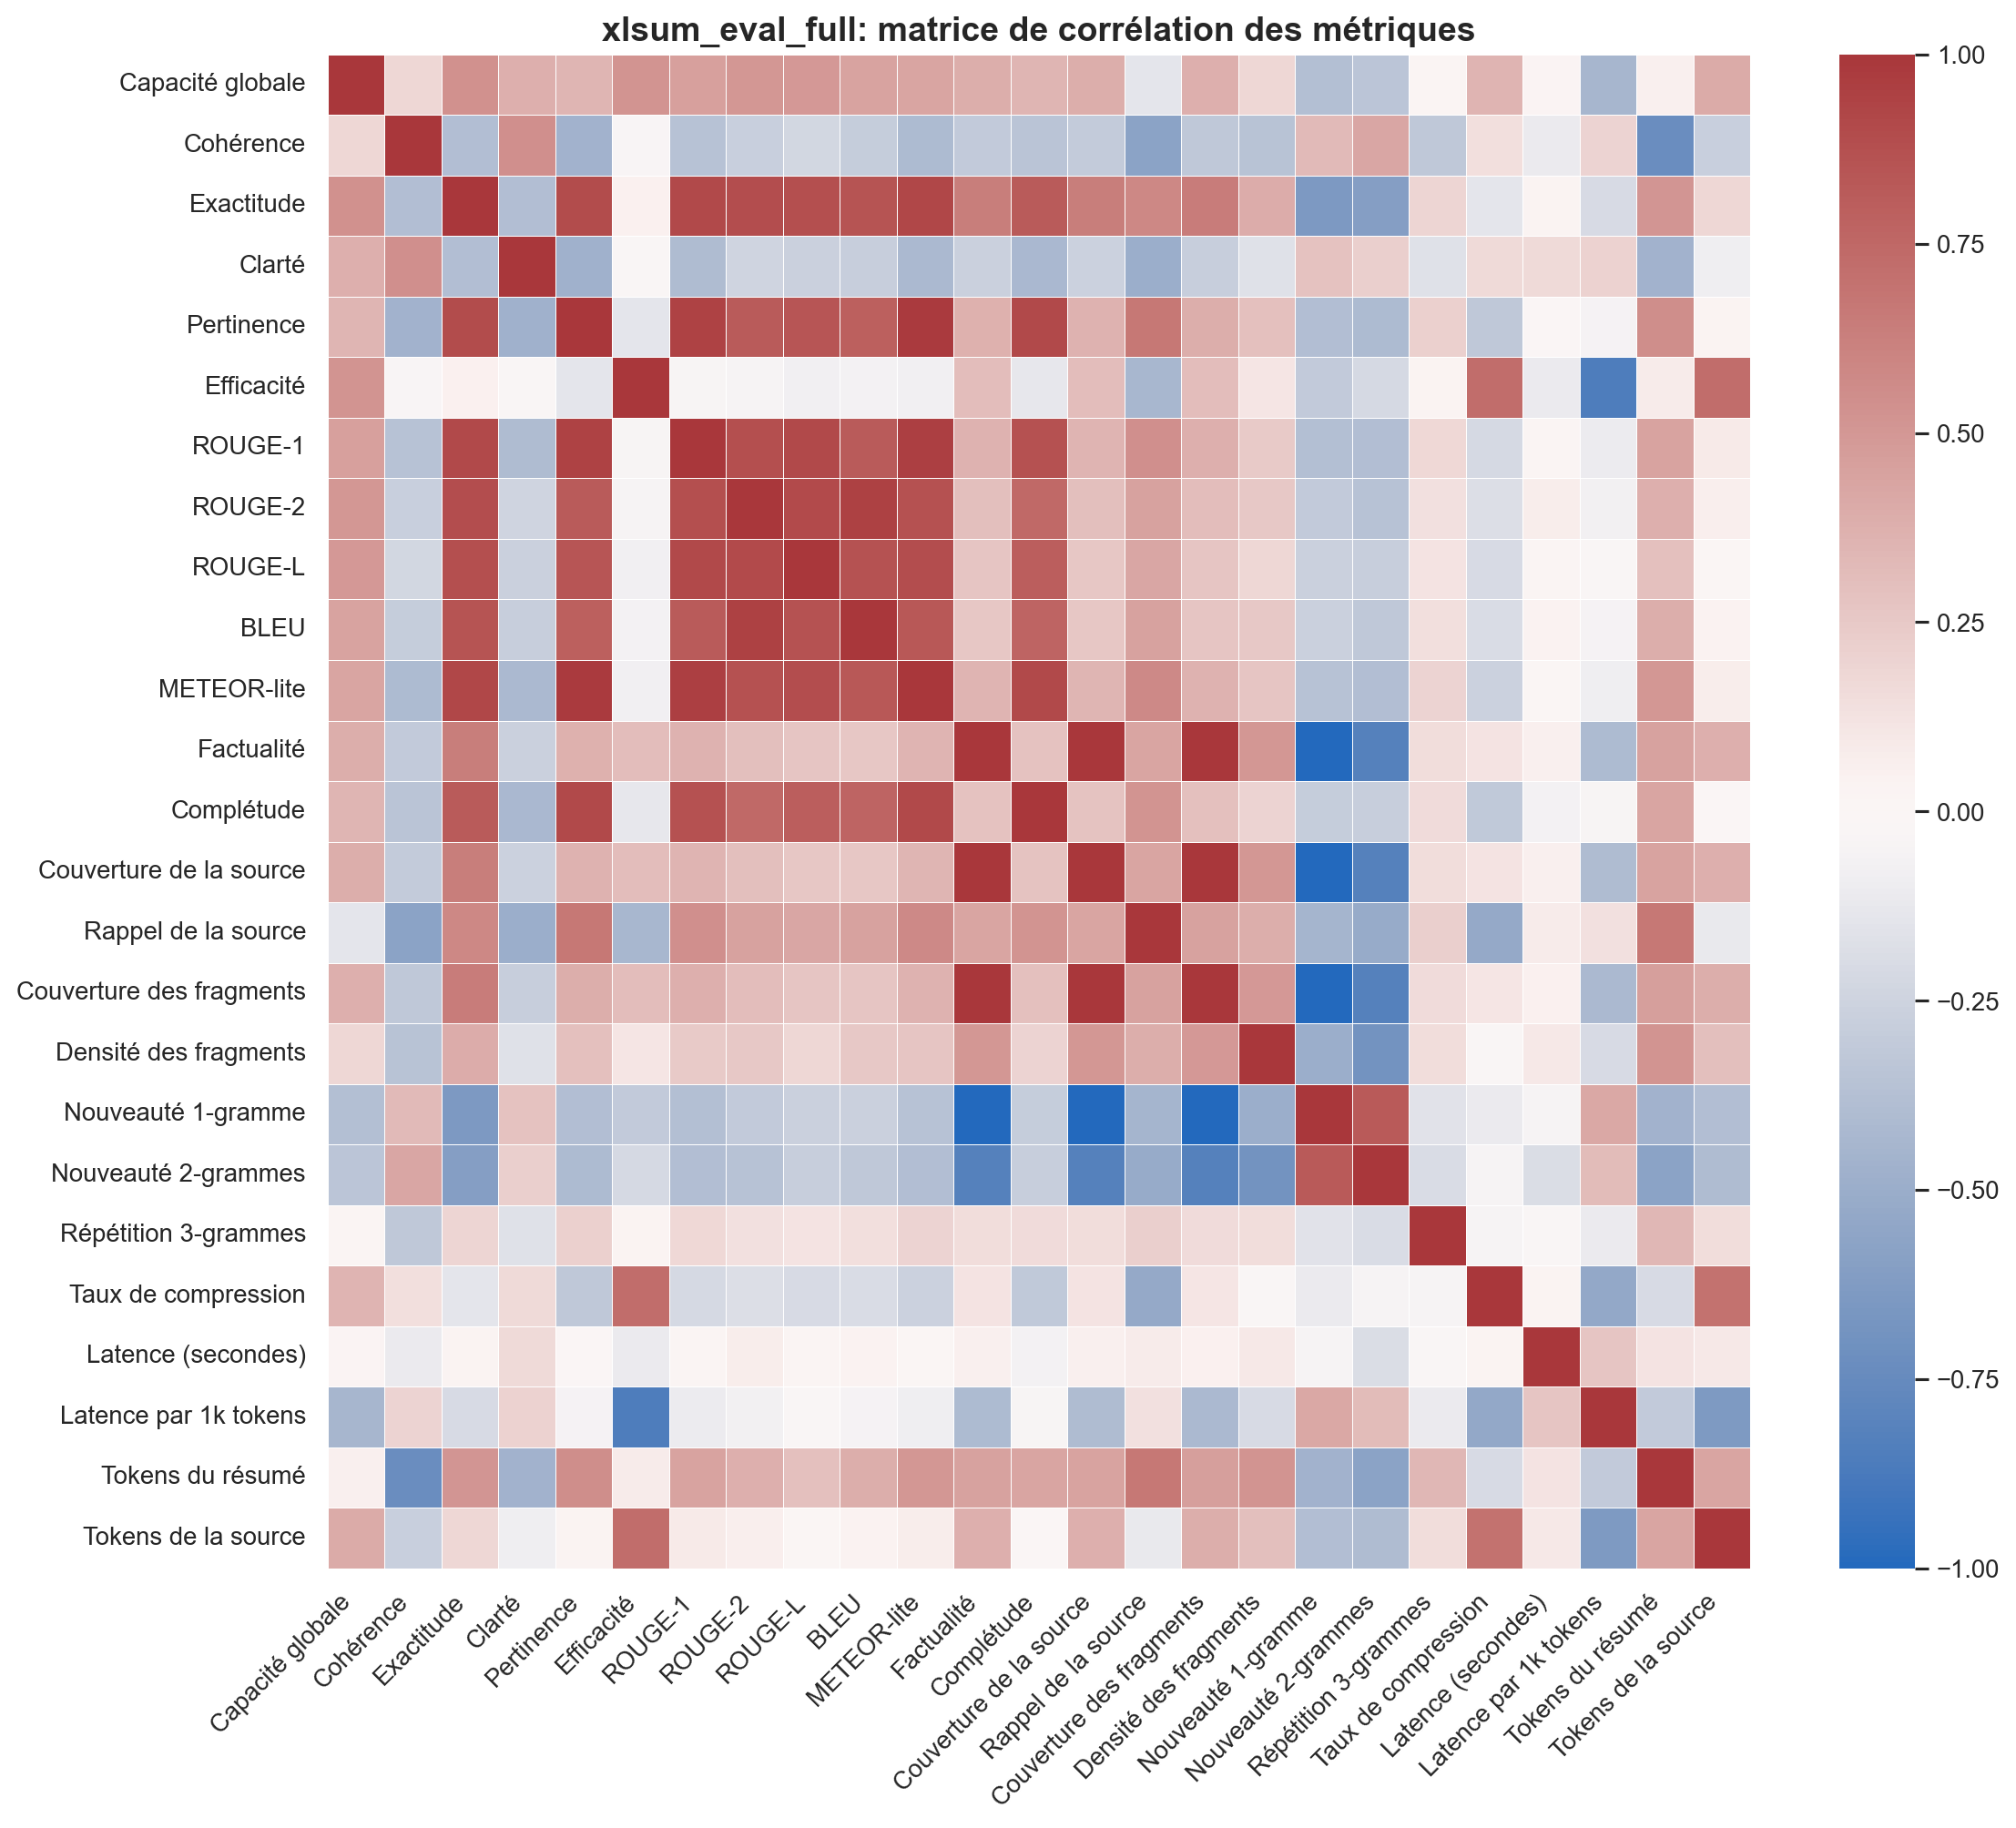
\includegraphics[width=.92\linewidth,height=.58\textheight,keepaspectratio]{figures/analyse/correlation_all_metrics.png}
\caption{Correlation entre les metriques d'evaluation}
\label{fig:analyse-correlation-all-metrics}
\vspace{0.6cm}
\begin{minipage}{.90\linewidth}
L'analyse des correlations confirme qu'il ne faut pas choisir le modele uniquement avec ROUGE-L. Un modele peut obtenir une meilleure similarite avec la reference tout en etant plus lent ou moins avantageux pour certaines contraintes applicatives. A l'inverse, un modele plus rapide peut perdre quelques points de similarite lexicale sans devenir inutilisable. La selection finale doit donc dependre du scenario: qualite textuelle maximale, fidelite a la source, vitesse, ou compromis entre ces dimensions.
\end{minipage}
\vspace*{\fill}
\end{figure}

Cette lecture explique aussi l'ecart entre les deux variantes mBART. Le premier modele est plus proche de la source: il a une couverture source moyenne de 0.8481 et une factualite automatique de 0.8522. Le second est plus abstrait: sa nouveaute 2-grammes monte a 0.4712, mais sa couverture source descend a 0.8203. Ainsi, \texttt{mbart-\allowbreak xlsum-2} reformule davantage, ce qui ameliore certaines metriques de completude et de recouvrement, mais diminue le signal de rattachement direct a l'article.

\section{Analyse exemple par exemple}

Les moyennes macro sont utiles, mais elles peuvent masquer des variations au niveau des exemples individuels. La Figure~\ref{fig:analyse-overall-win-rate} presente les taux de victoire exemple par exemple selon plusieurs metriques. Elle montre que la domination de \texttt{mt5-\allowbreak xlsum} dans les metriques classiques n'est pas absolue, meme si elle est nette.

\begin{figure}[t]
\centering
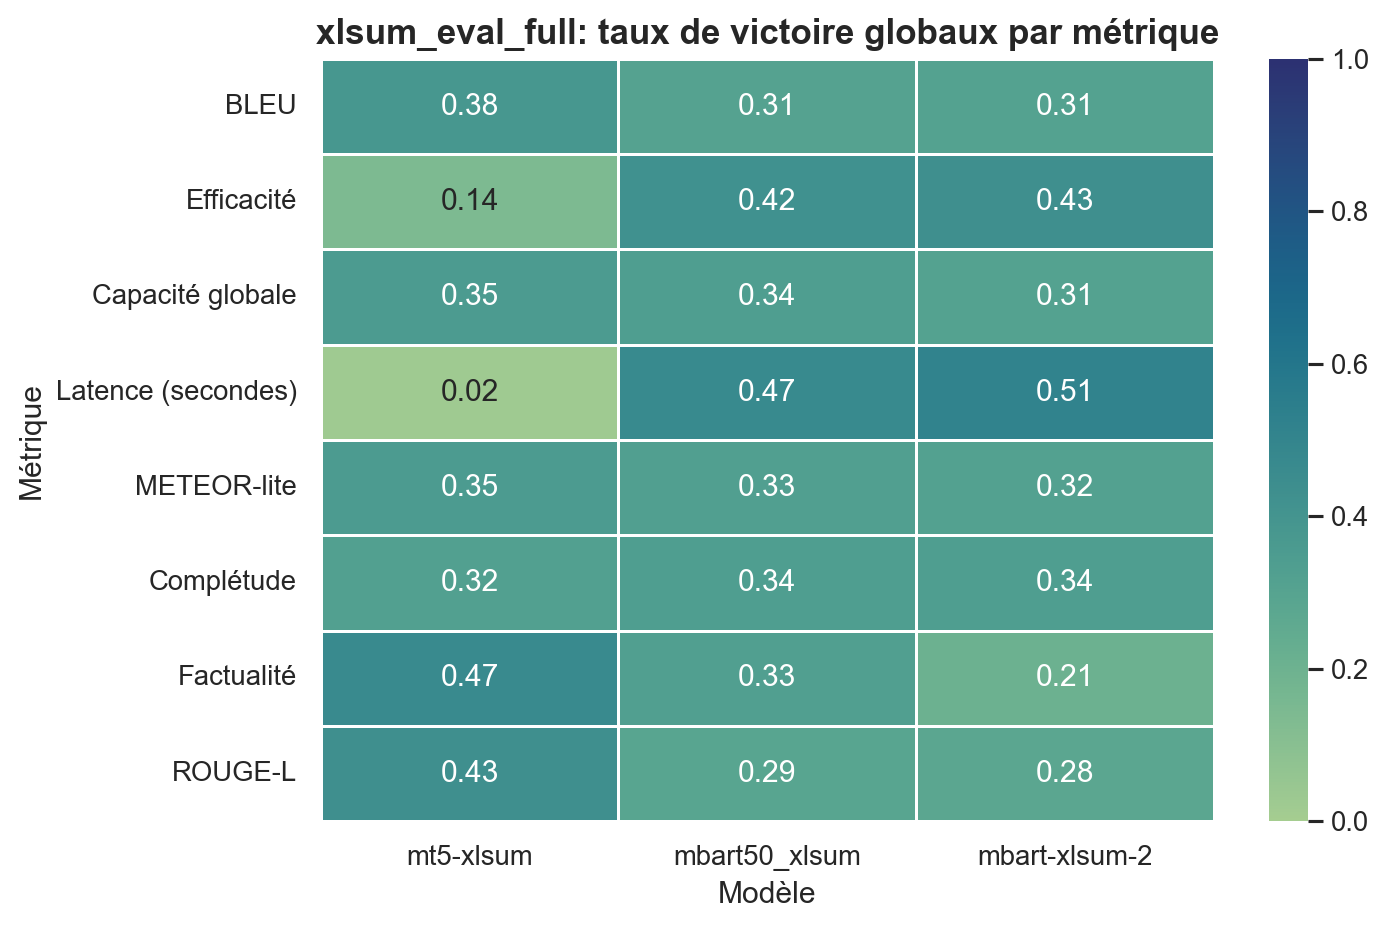
\includegraphics[width=.95\linewidth]{figures/analyse/overall_win_rate_by_metric.png}
\caption{Taux de victoire exemple par exemple selon les metriques}
\label{fig:analyse-overall-win-rate}
\end{figure}

\begin{table}[t]
\caption{Taux de victoire exemple par exemple dans l'evaluation complete}
\label{tab:analyse-win-rates}
\centering
\begin{tabular}{|l|r|r|r|}
\hline
\textbf{Metrique} & \textbf{\texttt{mt5}} & \textbf{\texttt{mbart50}} & \textbf{\texttt{mbart-2}} \\
\hline
Capacite globale & 35.4\% & 33.7\% & 30.9\% \\
\hline
ROUGE-L & 40.8\% & 28.7\% & 30.5\% \\
\hline
BLEU & 37.0\% & 30.3\% & 32.7\% \\
\hline
METEOR-lite & 34.1\% & 32.3\% & 33.6\% \\
\hline
Efficacite & 14.2\% & 42.4\% & 43.3\% \\
\hline
Completude & 30.1\% & 33.3\% & 36.6\% \\
\hline
Latence minimale & 1.4\% & 47.2\% & 51.4\% \\
\hline
\end{tabular}
\end{table}

Le Tableau~\ref{tab:analyse-win-rates} montre que \texttt{mt5-\allowbreak xlsum} gagne le plus souvent en ROUGE-L et BLEU. Cependant, les deux mBART gagnent tres majoritairement en latence et en efficacite. \texttt{mbart-\allowbreak xlsum-2} obtient aussi le meilleur taux de victoire en completude, avec 36.6\%. Cette analyse exemple par exemple confirme l'idee d'un compromis: \texttt{mt5-\allowbreak xlsum} est le plus fort pour la proximite au resume humain, mais les modeles mBART sont plus pratiques lorsque le cout de generation et la couverture utile sont prioritaires.

\section{Discussion sur le choix du modele}

Les resultats conduisent a trois conclusions principales. Premierement, \texttt{mt5-\allowbreak xlsum} est le meilleur modele si le critere principal est la similarite automatique avec les resumes de reference. Il est premier en ROUGE-L, BLEU, METEOR-lite, coherence, exactitude et clarte. Il constitue donc une reference solide pour l'evaluation du projet.

Deuxiemement, \texttt{mbart50\_\allowbreak xlsum} est le modele mBART le plus equilibre pour une utilisation applicative prudente. Son score global est tres proche de celui de \texttt{mt5-\allowbreak xlsum}, sa latence est plus faible, et sa fidelite a la source reste tres elevee. Dans un systeme de resume d'actualites, cette caracteristique est importante parce qu'un resume fluide mais trop eloigne de l'article peut produire une information trompeuse. Le choix de \texttt{mbart50\_\allowbreak xlsum} comme modele par defaut dans l'application est donc defendable si l'objectif est de privilegier la stabilite et l'ancrage source.

Troisiemement, \texttt{mbart-\allowbreak xlsum-2} est interessant lorsque l'on cherche un modele plus rapide et plus abstractive. Il obtient la meilleure efficacite, la meilleure completude automatique et la latence moyenne la plus basse. Cependant, sa baisse de \texttt{quality\_\allowbreak factuality} et de \texttt{source\_\allowbreak coverage} indique qu'il doit etre utilise avec attention pour les articles sensibles ou factuels.

Le Tableau~\ref{tab:analyse-model-choice} resume cette interpretation pratique des trois modeles.

\begin{table}[t]
\caption{Interpretation pratique des modeles}
\label{tab:analyse-model-choice}
\centering
\begin{tabular}{|p{2.8cm}|p{4.7cm}|p{4.7cm}|}
\hline
\textbf{Modele} & \textbf{Point fort principal} & \textbf{Usage recommande} \\
\hline
\texttt{mt5-\allowbreak xlsum} & Meilleure similarite avec les resumes de reference & Evaluation comparative et generation lorsque la qualite textuelle automatique est prioritaire. \\
\hline
\texttt{mbart50\_\allowbreak xlsum} & Bon compromis entre capacite, vitesse et fidelite a la source & Modele par defaut prudent pour l'application d'actualites multilingues. \\
\hline
\texttt{mbart-\allowbreak xlsum-2} & Meilleure vitesse et meilleure completude automatique & Scenario ou la latence, la couverture utile et la reformulation sont prioritaires. \\
\hline
\end{tabular}
\end{table}

\section{Limites de l'evaluation}

Les resultats doivent etre interpretes avec plusieurs limites. D'abord, les scores de coherence, exactitude, clarte, pertinence, efficacite, factualite et completude sont des proxies automatiques. Ils sont utiles pour comparer les modeles dans une meme pipeline, mais ils ne prouvent pas a eux seuls la qualite humaine ni la veracite factuelle des resumes.

Ensuite, l'evaluation est basee sur XL-Sum test. Ce corpus est adapte au resume d'actualites, mais il ne couvre pas toute la diversite des flux RSS reels utilises dans l'application. Les articles collectes en production peuvent etre plus bruyants, plus courts, plus longs, partiellement extraits ou structures differemment. Les performances observees sur XL-Sum ne garantissent donc pas exactement le meme comportement dans l'application.

Enfin, quatre langues du plan initial n'ont pas pu etre evaluees: allemand, italien, neerlandais et roumain. Elles restent presentes dans l'application, mais l'absence de sous-ensemble XL-Sum executable empeche une conclusion quantitative solide pour ces langues. Une prochaine etape serait de construire un jeu de test local pour ces langues, ou d'utiliser un autre corpus multilingue compatible avec la tache de resume.

\section{Conclusion de l'analyse}

L'evaluation complete montre que les modeles entraines dans le projet sont competitifs face a une reference mT5 deja specialisee. \texttt{mt5-\allowbreak xlsum} reste le meilleur modele en moyenne pour les metriques classiques et le score global, mais l'ecart avec \texttt{mbart50\_\allowbreak xlsum} est faible. Les modeles mBART apportent surtout un avantage applicatif: ils sont plus rapides et offrent un meilleur compromis entre cout de generation, completude et fidelite a la source.

Pour une utilisation finale dans le systeme de resume d'actualites, le choix le plus coherent est donc de ne pas resumer la performance par un seul score. \texttt{mt5-\allowbreak xlsum} doit rester une reference de qualite, \texttt{mbart50\_\allowbreak xlsum} est le candidat le plus prudent pour le mode par defaut, et \texttt{mbart-\allowbreak xlsum-2} peut etre propose comme alternative plus rapide et plus abstractive. Cette lecture par compromis correspond mieux aux contraintes d'une application reelle qu'un classement fonde uniquement sur ROUGE-L ou BLEU.
